\documentclass[12pt]{article}
\usepackage{amsmath}
\usepackage{amsthm}
\usepackage{graphicx,psfrag,epsf}
\usepackage{enumerate}
\usepackage{natbib}
\usepackage{url} % not crucial - just used below for the URL

%\pdfminorversion=4
% NOTE: To produce blinded version, replace "0" with "1" below.
\newcommand{\blind}{0}

% DON'T change margins - should be 1 inch all around.
\addtolength{\oddsidemargin}{-.5in}%
\addtolength{\evensidemargin}{-.5in}%
\addtolength{\textwidth}{1in}%
\addtolength{\textheight}{1.3in}%
\addtolength{\topmargin}{-.8in}%


%%%% Packages and definitions
\usepackage{amssymb}

\usepackage{xr}

\usepackage[top=0.85in,left=1.0in,right=1.0in,footskip=0.75in]{geometry}

% Use adjustwidth environment to exceed column width (see example table in text)
\usepackage{changepage}

% Use Unicode characters when possible
\usepackage[utf8]{inputenc}

% textcomp package and marvosym package for additional characters
\usepackage{textcomp,marvosym}

\usepackage[ruled]{algorithm}
\usepackage{algorithmic}

% cite package, to clean up citations in the main text. Do not remove.
\usepackage{cite}

% Use nameref to cite supporting information files (see Supporting Information section for more info)
\usepackage{nameref,hyperref}

%\usepackage{amsthm}

% ligatures disabled
\usepackage{microtype}
\DisableLigatures[f]{encoding = *, family = * }

% for the beautiful checkmarks
\usepackage{pifont}

\newtheorem{theorem}{Theorem}
\newtheorem{corollary}{Corollary}
\newtheorem{lemma}{Lemma}
\newtheorem{definition}{Definition}
\newtheorem{condition}{Condition}

\DeclareMathOperator*{\argmin}{arg\,min}


\begin{document}

\def\spacingset#1{\renewcommand{\baselinestretch}%
{#1}\small\normalsize} \spacingset{1}


%%%%%%%%%%%%%%%%%%%%%%%%%%%%%%%%%%%%%%%%%%%%%%%%%%%%%%%%%%%%%%%%%%%%%%%%%%%%%%

\if0\blind
{
  \title{\bf Oracle Inequalities for multiple penalty parameters}
  \author{Jean Feng\thanks{
    Jean Feng was supported by NIH grants ???. % DP5OD019820 and T32CA206089.
    Noah Simon was supported by NIH grant DP5OD019820.
    The content is solely the responsibility of the authors and does not necessarily represent the official views of the National Institutes of Health.}\\
    Department of Biostatistics, University of Washington\\
    and \\
    Noah Simon \\
    Department of Biostatistics, University of Washington}
  \maketitle
} \fi

\if1\blind
{
  \bigskip
  \bigskip
  \bigskip
  \begin{center}
    {\LARGE\bf Cross-validation for many penalty parameters.}
\end{center}
  \medskip
} \fi

\bigskip
\begin{abstract}

In penalized regression problems, the choice of penalty parameters is important since they ultimately determine the fitted model. The penalty parameters that minimize the generalization error are generally unknown and must be estimated. In this paper, we establish finite-sample oracle inequalities for penalty parameters selected by either a training/validation split framework or cross-validation. We show that if the fitted models are smoothly parameterized by the penalty parameters, the upper bound of the model error depends on the oracle error and a near-parametric term. This near-parametric term roughly corresponds to the error from tuning penalty parameters. In semi- or non-parametric problems, the upper bound is generally dominated by the oracle error and, in fact, the number of penalty parameters can grow with the sample size without affecting the asymptotic convergence rate.

\end{abstract}

\noindent%
{\it Keywords:}  Regression, Cross-validation, Regularization
\vfill

\newpage
\spacingset{1.45}
\section{Introduction}

Per the usual regression framework, we observe response $y \in \mathbb{R}$ and predictors $\boldsymbol {x} \in \mathbb{R}^p$. Suppose $y$ is generated from the model $g^*$ from model class $\mathcal{G}$
\begin{equation}
y = g^*(\boldsymbol x) + \epsilon
\end{equation}
where $\epsilon_i$ are random errors. Our goal is to find the best model in $\mathcal{G}$ to model $y$ given $\boldsymbol x$.

In high-dimensional ($p \gg n$) or ill-posed problems, the ordinary least squares estimate performs poorly as it overfits to the training data. A common solution is to add regularization, or penalization, to control model complexity and induce desired structure. The penalized least squares estimate minimizes a criterion of the form
\begin{equation}
\label{intro_train_criterion}
\hat{g}(\cdot | \boldsymbol \lambda) = \argmin_{g\in \mathcal{G}} \frac{1}{n} \sum_{i=1}^n \left (y_i -  g(x_i) \right )^2 + \sum_{j=1}^J \lambda_j P_j(g)
\end{equation}
where $P_j$ are the penalty functions and $\lambda_j$ are the penalty parameters.

Selecting the penalty parameters is an important task since they ultimately determine the fitted model. Their oracle values balance the residual least squares and the penalty terms to ensure fast convergence rates \citep{van2000empirical}. For example, when fitting an additive model $f(\boldsymbol x) = \sum_{j=1}^J f_j(x_j)$ with a roughness penalty for each component, the penalty parameters should be inversely proportional to the penalties of the true model \citep{van2014additive}. When fitting a linear model using the lasso, the penalty parameter should be on the order $\sigma (\log p /n )^{1/2}$ where $\sigma^2$ is the variance of the error terms \citep{buhlmann2011statistics}.

The obvious problem is that the oracle penalty parameters depend on unknown values. Thus penalty parameters are usually tuned via a training/validation split or cross-validation. The basic idea is to train a model on a random partition of the data and evaluate its error on the remaining data. One then searches for the penalty parameters that minimize the error on this validation set. For a more complete review of cross-validation, refer to Arlot \citep{arlot2010survey}.

The performance of cross-validation-like procedures is characterized by bounding the prediction error. Typically the upper bound is composed of two terms: the error of the oracle plus a complexity term. In a general cross-validation framework, \citet{van2003unified, van2004asymptotic} provides finite sample oracle inequalities assuming that cross-validation is performed over a finite model class and \citet{lecue2012oracle} uses an entropy approach to bound the error for cross-validated models from potentially infinite model classes. In the regression setting, \citet{gyorfi2006distribution} provides a finite sample inequality for training/validation split for least squares and \citet{wegkamp2003model} proves an oracle inequality for a penalized least squares holdout procedure. There are also bounds for cross-validated models from ridge regression and lasso \citep{golub1979generalized, chetverikov2016cross, chatterjee2015prediction}, though the proofs usually rely on the linearity of the model class and are therefore hard to generalize.

Despite the wealth of literature on cross-validation, there is very little work on characterizing the prediction error when the regularization method has multiple penalty parameters. A potential reason is that tuning multiple penalty parameters is computationally difficult so most regularization methods only have one or two tuning parameters, such as the Elastic Net and Sparse Group Lasso \citep{zou2003regression, simon2013sparse}. However, recent efforts have made this ``hyperparameter selection" problem computationally tractable by using continuous optimization methods. For penalized regression problems, the gradient of the validation loss with respect to the penalty parameters can often be calculated using an implicit differentiation trick \citep{bengio2000gradient, foo2008efficient}. Thus a gradient descent procedure can be used to tune the penalty parameters. For more general machine learning problems, one can use a gradient-free approach such as Bayesian optimization \citet{snoek2012practical}.

This paper provides a finite-sample upper bound on the prediction error when multiple penalty parameters are tuned via a training/validation split or cross-validation. We first show that if the fitted functions vary smoothly in the penalty parameters, then the difference between the error of the selected model and the oracle model shrinks at a near-parametric rate. Next we show that this smoothness assumption is satisfied by many penalized regression problems. Our result suggests that the prediction error can be minimized by either appropriately increasing the number of penalty parameters or shrinking the validation set size as the sample size grows. The proofs rely on empirical process theory and the implicit differentiation trick in \citet{bengio2000gradient} and \citet{foo2008efficient}.

Section \ref{sec:main_results} provides bounds on the prediction error for a training/validation framework and cross-validation.
Section \ref{sec:entropy} proves that for many penalized regression problems, the fitted models are smoothly parameterized by the penalty parameters.
Section \ref{sec:simulations} provides a simulation study to support our theoretical results.
Section \ref{sec:discussion} discusses our findings and potential future work.
Section \ref{sec:proofs} contains the proofs and other technical details.

\section{Main Result} \label{sec:main_results}

\subsection{Training/Validation Split}

Given the total observed dataset $D$ of size $n$, suppose it is randomly split into a training set $T$ of size $n_T$ and validation set $V$ of size $n_V$. For a function $h$, define $\| h \|_V^2 = \frac{1}{n_V}\sum_{i\in V} h^2(x_i)$ and similarly for $T$. Using this notation, the fitted model defined in  \eqref{intro_train_criterion} can be reformulated as
\begin{equation}
\hat{g}(\cdot | \boldsymbol \lambda) = \argmin_{g\in \mathcal{G}} \frac{1}{2} \left \|y -  g \right \|_T^2 + \sum_{j=1}^J \lambda_j P_j(g)
\end{equation}
In the training/validation framework, the selected penalty parameters minimize the validation error as follows
\begin{equation}
\label{cv_lambda}
\hat{\boldsymbol \lambda} = \arg\min_{\lambda\in\Lambda} \frac{1}{2} \left \| y-\hat{g}(\cdot | \boldsymbol \lambda) \right \|_{V}^{2}
\end{equation}
where $\Lambda$ is the range of penalty parameter values. We are interested in bounding the difference between the fitted model and the true model at the observed covariates in the validation set, which can be expressed as $\left \|\hat{g}(\cdot | \hat{\boldsymbol \lambda}) - g^* \right \|_V$.

Our bound is based on the basic inequality \citep{van2000empirical}. Let the oracle penalty parameters $\tilde{\boldsymbol \lambda}$ be defined as
\begin{equation}
\tilde{\boldsymbol \lambda} = \argmin_{\lambda \in \Lambda} \frac{1}{2} \left \| \hat{g}(\cdot | \tilde{\boldsymbol \lambda}) - g^* \right \|^2
\end{equation}
where $\| h \| = \int h^2(x) d\mu(x)$. Let the set of fitted models be denoted
\begin{equation}
\label{function_class_GT}
\mathcal{G}(T) = \left \{ \hat{g}(\cdot | \boldsymbol \lambda) : \lambda \in \Lambda  \right \}
\end{equation}
From the definition of $\hat{\boldsymbol \lambda}$, we have
\begin{eqnarray}
\label{basic_ineq}
\left \|\hat{g}(\cdot | \hat{\boldsymbol \lambda}) - g^* \right \|_V^2
& \le &
\left \| \hat{g}(\cdot | \tilde{\boldsymbol \lambda}) - g^* \right \|_V^2 +
2 \left \langle \epsilon, \hat{g}(\cdot | \hat{\boldsymbol \lambda}) - \hat{g}(\cdot | \tilde{\boldsymbol \lambda}) \right \rangle_V \\
& \le &
\left \| \hat{g}(\cdot | \tilde{\boldsymbol \lambda}) - g^* \right \|_V^2 +
\sup_{g \in \mathcal{G}(T)} 2 \left \langle \epsilon, g - \hat{g}(\cdot | \tilde{\boldsymbol \lambda}) \right \rangle_V
\end{eqnarray}
where $\langle h, \ell \rangle_A = \frac{1}{size(A)}\sum_{i\in A} h(x_i) \ell(x_i)$. This upper bound can be understood as a bias-variance tradeoff. The first term is the difference between the oracle model and the truth, so this is just the bias from using the model class $\mathcal{G}(T)$. The second term is an empirical process term that can be bounded by its variance, so this can be thought of as the ``variance" of $\mathcal{G}(T)$.

Empirical process theory provides a more formal framework for characterizing the behavior of the empirical process term. ``Variance" is usually referred to as complexity and can be measured in a number of ways; we will use metric entropy in this paper. A more thorough review of empirical process theory is presented in Section \ref{sec:proofs}. Here we only highlight the fact that functions smoothly parameterized by $\boldsymbol \theta$ as follows
\begin{equation}
\left \| f(\cdot | \boldsymbol \theta) - f(\cdot | \boldsymbol \theta') \right \|
\le
O_p \left (\| \boldsymbol \theta - \boldsymbol \theta' \|_2 \right ) 
\end{equation}
have low metric entropy. Hence their empirical process terms are small with high probability.

In the penalized regression setting, the fitted functions $\hat{g}(\cdot | \boldsymbol \lambda)$ are parameterized by $\boldsymbol \lambda$. Moreover, we show in Section \ref{sec:entropy} that $\hat{g}(\cdot | \boldsymbol \lambda)$ is smoothly parameterized by $\boldsymbol \lambda$ for many penalized regression problems. This fact combined with \eqref{basic_ineq} provides a finite-sample upper bound on the error of the fitted model $\hat{g}_{\hat \lambda}(\cdot | T)$ over the validation points.

\begin{theorem}
\label{train_val_thrm}
Suppose that $\sup_{g \in \mathcal{G(\cdot | T)}} \| g \|_\infty \le G < \infty$.
Suppose that $\Lambda = [ n_V^{-t_{\min}}, n_V^{t_{\max}} ]^J $.

Suppose that if $\| \epsilon \|_T \le 2 \sigma $, there is some constant $C, \kappa$ such that for any $u> 0$, we have
\begin{equation}
\left \| \hat{g}(\cdot | \boldsymbol \lambda_1) - \hat{g}(\cdot | \boldsymbol \lambda_2) \right \|_V 
\le 
\frac{1}{C} n^{-\kappa} \left \| \boldsymbol \lambda_1 - \boldsymbol \lambda_2 \right \|
\end{equation}

Then with high probability, we have for constants $c_1, c_2$
\begin{equation}
\label{error_bound}
\left\Vert \hat{g}(\cdot | \hat{\lambda}) -g^{*}\right\Vert _{V} 
\le
\|\hat{g}(\cdot | \tilde{\lambda} ) -g^{*}\|_{V}
+c_{1} \left (\frac{J(\log n_{V}+c_{2})}{n_{V}} \right )^{1/2}
+\sqrt{ c_{1} \left (\frac{J(\log n_{V}+c_{2})}{n_{V}} \right )^{1/2} \|\hat{g}(\cdot | \tilde{\lambda} ) -g^{*}\|_{V}}
\end{equation}
\end{theorem}
Theorem \ref{train_val_thrm} is a special case of Theorem \ref{train_val_thrm_complicated} and their proofs are given in Section \ref{sec:proofs}.

The $\log n_V$ terms are the result of increasing the range of $\Lambda$ at a polynomial rate. Increasing the range of $\Lambda$ in important to ensure fast convergence rates.



\subsection{Cross-Validation}

In practice, $K$-fold cross-validation is a far more common procedure than a training/validation split. In addition, we will now bound the generalization error rather than the prediction error over the validation observations. Toward this end, we will apply the oracle inequality in \citet{lecue2012oracle} to the problem of penalized regression.

The problem setup for $K$-fold CV is as follows. Let the $K$ partitions for $k=1,...,K$ be denoted $D_k$ (with size $n_k$) and the entire set minus the $D_k$ will be denoted $D_{-k}$. Consider the joint optimization problem for $K$-fold CV:
\begin{eqnarray}
\label{kfold_opt}
\hat{\boldsymbol \lambda} &=& \arg\min_{\lambda\in\Lambda} \frac{1}{2K} \sum_{k=1}^K  \| y-\hat{g}_{k}(\cdot | \boldsymbol \lambda) \|_{D_k}^{2} \\
\hat{g}_{k}(\cdot | \boldsymbol \lambda) &=&\arg\min_{g\in\mathcal{G}} \frac{1}{2} \| y-g \|_{D_{-k}}^{2} + \sum_{j=1}^J \lambda_j P_j(g)
\end{eqnarray}

In traditional cross-validation, the final model is retrained on all the data with $\hat{\lambda}$. However, bounding its generalization error requires additional regularity assumptions \citep{lecue2012oracle}. We consider the following ``averaged version of cross-validation" instead
\begin{equation}
\hat{g}_{ACV}(\cdot) = \frac{1}{K} \sum_{k=1}^K \hat{g}_{k}
(\cdot | \hat{\boldsymbol \lambda})
\end{equation}
The following theorem bounds the generalization error of $\hat{g}_{ACV}$.

\begin{theorem}
\label{kfold_thrm}

Suppose the errors have expectation zero and $\| \epsilon \|_\infty < \infty $.

Suppose $\sup_{g \in \mathcal{G}} \|g\|_\infty \le G$.

Suppose there are constants $C, \kappa$ such that
\begin{equation}
\| \hat{g}(\cdot | \boldsymbol \lambda_1) - \hat g (\cdot | \boldsymbol \lambda_2) \|_\infty \le \frac{1}{C} n^{-\kappa} \| \boldsymbol \lambda_1 - \boldsymbol \lambda_2 \| 
\end{equation}
Suppose that $\Lambda = [ n^{-t_{\min}}, n^{t_{\max}} ]^J $.


With high probability, we have for any $a > 0$,
\begin{equation}
\label{smooth_error_bound}
E_{D} \left \| \hat{g}_{ACV} - g^* \right \|^2 \le
(1+a) \min_{k\in 1:K, \lambda \in \Lambda}  E_{D} \left \| \hat{g}_k(\cdot |\boldsymbol \lambda) - g^* \right \|^2
+ c_a \max_{k=1:K} \frac{\log^2(n)}{n_k}
\end{equation}
where $c_a$ is given in Mitchell.
\end{theorem}


Theorem \ref{kfold_thrm} is a stronger result than Theorem \ref{train_val_thrm}, but one is required to show that $\hat{g}_\lambda$ is smoothly parameterized by $\lambda$ over the entire domain, not just the validation points.

\subsubsection{Example}

We present a nonparametric additive model as an example.

Consider the training criterion with Sobolev penalties on each of the components
\begin{equation}
\hat{f}(\cdot | {\boldsymbol \lambda}), \hat{g}(\cdot | {\boldsymbol \lambda}) =
\argmin_{f,g \in \mathcal{G}}
\| y - (f + g) \|_n^2 +
\lambda_1 \int_0^1 |f^{(s)}(x)|^2 dx +
\lambda_2 \int_0^1 |g^{(t)}(x)|^2 dx
\end{equation}
where $\mathcal{G}$ are functions defined over the domain [0,1].
It can be shown that the estimate is a spline. According to \citet{van2014additive}, the oracle convergence rate is
\begin{equation}
\| \hat{f}(\cdot | \tilde{\boldsymbol{\lambda}}) - f^* \| = O_p(n^{-\frac{s}{2s+1}}),
\| \hat{g}(\cdot | \tilde{\boldsymbol{\lambda}}) - g^* \| = O_p(n^{-\frac{t}{2t+1}})
\end{equation}
However, one would need to know the Sobolev penalties of $f^*$ and $g^*$ in order
to determine the oracle penalty parameters.
If the penalty parameters are chosen using the training/validation framework, Theorem \ref{train_val_thrm} gives us
\begin{eqnarray*}
\| \hat{f}(\cdot | \hat{\boldsymbol{\lambda}}) + \hat{g}(\cdot | \hat{\boldsymbol{\lambda}}) - (f^* + g^*) \|_V &=&
O_p(n_T^{-\frac{s}{2s+1}}) + O_p(n_T^{-\frac{t}{2t+1}})
+c_{1} \left (\frac{J(\log n_{V}+c_{2})}{n_{V}} \right )^{1/2} \\
&& +\sqrt{ c_{1} \left (\frac{J(\log n_{V}+c_{2})}{n_{V}} \right )^{1/2}  \left (O_p(n_T^{-\frac{s}{2s+1}}) + O_p(n_T^{-\frac{t}{2t+1}}) \right) }
\end{eqnarray*}
If the penalty parameters are chosen instead using a $K$-fold cross-validation framework, Theorem \ref{kfold_thrm} states that the
averaged version of cross-validation has a generalization error that is bounded as follows
\begin{eqnarray*}
E_D \| \hat{f}_{ACV} + \hat{g}_{ACV} - (f^* + g^*) \|^2 &=&
(1+a) E_D  \left (O_p(n_k^{-\frac{s}{2s+1}}) + O_p(n_k^{-\frac{t}{2t+1}})  \right )
+ c_a \max_{k=1:K} \frac{\log^2(n)}{n_k}
\end{eqnarray*}

\subsubsection{Implications}
Theorem \ref{train_val_thrm} and \ref{kfold_thrm} imply that $\hat{g}(\cdot | \hat{\boldsymbol{\lambda}})$ has a semi-parametric convergence rate: the nonparametric (or potentially parametric) convergence rate of the oracle and the parametric convergence rate of the cross-validated model to the oracle. As long as the number of penalty parameters is finite, it does not affect the convergence rate of the model asymptotically.

We can minimize the prediction error by balancing the two terms in the upper bound. The inequalities suggest that there are many approaches. One could change increase the training to validation ratio as the sample size grows. Alternatively, one could increase the number of penalties and penalty parameters with the number of samples. Of course, finding the true minimizer of the upper bound will require knowing properties about the true model, so this would have to be done in some heuristic manner.

\section{Smoothness of $\hat{g}(\cdot | \boldsymbol{\lambda})$ in $\boldsymbol \lambda$}
\label{sec:entropy}

We now show that $\hat{g}(\cdot | \boldsymbol{\lambda})$ is smoothly parametrized by $\lambda$. Theorem \ref{train_val_thrm} requires this smoothness assumption to hold over the validation observations whereas Theorem \ref{kfold_thrm} requires this to hold over the entire domain. Smoothness over the validation set is generally easier to show. We will prove it for nonparametric additive models with smooth penalties and certain nonsmooth penalties. Smoothness over the entire domain is harder to show, so we consider two specific examples: parametric regression problems (where $p$ can grow with $n$) and smoothing splines.

Throughout, we will presume that $\mathcal{G}$ is a convex function class.

\subsection{Smoothness over the Validation Set}
\label{sec:smoothness_validation}
We will show that $\hat{g}(\cdot | \boldsymbol{\lambda})$ varies smoothly with respect to $\lambda$ over the observed covariates, which will directly imply smoothness over the validation set. Suppose we are in the additive model setting. The fitted models minimize the training criterion
\begin{equation}
\label{orig_train_criterion}
\left\{ \hat{g}_j(\cdot | \boldsymbol \lambda) \right \}_{j=1}^J = \argmin_{g\in \mathcal{G}} \| \boldsymbol y -  \sum_{j=1}^J g_j(\boldsymbol x_j) \|^2_T + \sum_{j=1}^J \lambda_j P_j(g_j)
\end{equation}

We will not directly consider functions that minimize \eqref{orig_train_criterion}. Instead we will characterize the function class that minimize the perturbed training criterion
\begin{equation}
\label{train_crit_ridge}
\left\{ \hat{g}_j(\cdot | \boldsymbol \lambda) \right \}_{j=1}^J = \argmin_{g\in \mathcal{G}} \| \boldsymbol y -  \sum_{j=1}^J g_j(\boldsymbol x_j) \|^2_T + \sum_{j=1}^J \lambda_j \left ( P_j(g_j) + \frac{w}{2} \| g_j \|^2_D \right )
\end{equation}
where $w > 0$ is some constant. The additional ridge penalty will be used in the proofs to ensure that the model is ``well-conditioned" over the observed covariates.

In practice, one can choose $w$ to be small enough such that the fitted models from \eqref{train_crit_ridge} are indistinguishable from those in \eqref{orig_train_criterion}. Lemma \ref{oracle_maintained} proves that the convergence rate of the oracle penalty parameters is preserved for small enough $w$.

\subsubsection{Smooth Penalties}
We will first consider the simple case where the penalties $P_j$ are twice-differentiable everywhere. The following lemma shows that fitted function values vary smoothly in the penalty parameters.

\begin{lemma}
\label{lemma:smooth}
We suppose the penalty functions $P_{j}$ are convex and twice-differentiable.
Suppose that $\sup_{g\in\mathcal{G}}\|g\|_{D}\le G$.
Suppose $\lambda_j \ge \lambda_{\min}$ for all $j$.

%For all $d>0$, any $\boldsymbol \lambda^{(1)}, \boldsymbol \lambda^{(2)}$ that satisfy
%\[
%\|\boldsymbol \lambda^{(1)}- \boldsymbol \lambda^{(2)}\|\le\frac{dw}{2J}\left(\frac{n}{n_T \lambda_{\min} }\left(2G+\|\epsilon\|_{T}\right)+wG+G\right)^{-1}\lambda_{\min}
%\]

For all $\boldsymbol \lambda^{(1)}, \boldsymbol \lambda^{(2)} \in \Lambda$, we have
\[
\left \|
\sum_{j=1}^{J}\hat{g}_{j}(\cdot| \boldsymbol \lambda^{(1)})-\hat{g}_{j}(\cdot| \boldsymbol \lambda^{(2)})
\right \|_{D}
\le
\frac{2J}{w\lambda_{\min}}\left(\frac{n}{n_T \lambda_{\min} }\left(2G+\|\epsilon\|_{T}\right)+wG+G\right) 
\left \|
\boldsymbol \lambda^{(1)}- \boldsymbol \lambda^{(2)}
\right \|
\]
\end{lemma}

All of the proofs on the smoothness of $\hat{g}(\cdot | \boldsymbol \lambda)$ follow the same recipe. The first step is to consider the optimization problem \eqref{orig_train_criterion} restricted to models on the line
\begin{equation}
\left \{ \hat{g}(\cdot |\boldsymbol \lambda^{(1)}) + m \left (\hat{g}(\cdot |\boldsymbol \lambda^{(2)})  - \hat{g}(\cdot |\boldsymbol \lambda^{(1)}) \right ) : m \in [0,1] \right \}
\end{equation}
By implicit differentiation of the KKT conditions, we can then determine how the fitted models change with respect to the penalty parameters. Finally, the difference $\| \hat{g}(\cdot | \boldsymbol \lambda^{(1)}) -  \hat{g}(\cdot | \boldsymbol \lambda^{(2)}) \|$ is bounded using the mean value theorem. Depending on the situation, the result can be proven directly or by contradiction.

For illustration, we present the proof for Lemma \ref{lemma:smooth} in the case where there is only one penalty parameter. The case with multiple penalty parameters is given in Section \ref{sec:proofs}.

\begin{proof}[Proof of Lemma \ref{lemma:smooth}]

Let $h=\hat{g}(\cdot|\lambda^{(1)})-\hat{g}(\cdot|\lambda^{(2)})$. Suppose for contradiction that $\|h\|_{D} > d$.
Consider the one-dimensional optimization problem
\[
\hat{m}(\lambda) = \arg\min_{m}\frac{1}{2}\|y- \left(g +mh\right)\|_{T}^{2}+\lambda\left(P(g+mh)+\frac{w}{2}\|g+mh\|_{D}^{2}\right)
\]

Now by the KKT conditions, we have
\[
\langle y-\left(g+mh\right),h\rangle_{T}+\lambda\frac{\partial}{\partial m}P(g+mh)+\lambda w \langle h,g+mh\rangle_{D}=0
\]


It's implicit derivative with respect to $\lambda$ is
\begin{equation}
 \frac{\partial\hat{m}(\lambda)}{\partial\lambda}  =
\left ( \| h\|_{T}^2 +\lambda\frac{\partial^{2}}{\partial m^{2}}P(g+mh) +\lambda w\|h\|_{D}^{2} \right )^{-1}
\left ( \frac{\partial}{\partial m}P(g+mh)+w\langle h,g+mh\rangle_{D} \right )
\end{equation}

From the KKT conditions, we can show
\[
\left | \frac{\partial}{\partial m}P(g+mh) \right |  \le
\left(\frac{n}{n_{T} \lambda_{\min}}\left(2G+\|\epsilon\|_{T}\right)+wG+G\right)  \|h\|_{D}
\]
Hence
\[
\left|\frac{\partial}{\partial\lambda}\hat{m}(\lambda)\right| \le
\left(\frac{n}{n_{T}}n^{\tau_{min}}\left(2G+\|\epsilon\|_{T}\right)+wG+G\right)n^{\tau_{\min}}w^{-1}\|h\|_{D}^{-1}
\]

By the MVT, there is some $\alpha\in (\lambda^{(1)},\lambda^{(2)})$ such that
\begin{eqnarray*}
\left|\hat{m}(\lambda^{(2)})-\hat{m}(\lambda^{(1)})\right| & = &
\left|\left ( \lambda^{(2)}-\lambda^{(1)} \right )
\left . \frac{\partial \hat{m}(\lambda) }{\partial\lambda}\right |_{\lambda=\alpha} \right|\\
 & \le & |\lambda^{(2)}-\lambda^{(1)}|
\left(\frac{n}{n_{T} \lambda_{\min} }\left(2G+\|\epsilon\|_{T}\right)+wG+G\right)\frac{1}{wd \lambda_{\min} } \\
 & = & 1/2
\end{eqnarray*}


But this is a contradiction since we know that $\hat{m}(\lambda^{(2)})=1$
and $\hat{m}_{\tilde{k}}(\lambda^{(1)})=0$.
\end{proof}

\subsubsection{Nonsmooth penalties}\label{sec:nonsmooth}

If the regression problem contains non-smooth penalty functions, similar results do not necessarily hold. Nonetheless, we find that for many popular non-smooth penalty functions, the functions $\hat{g}(\cdot | \boldsymbol \lambda)$ are still smoothly parameterized by $\boldsymbol \lambda$ almost everywhere. To characterize such problems, we use the approach in Feng \& Simon (TBD- CITE?). We begin with the following definitions:

\begin{definition}
The differentiable space of a real-valued function $L$ at $g \in \mathcal{G}$ is the set of functions
\begin{equation}
\Omega^{L}(g) = \left \{ h \in \mathcal{G} \middle | \lim_{\epsilon \rightarrow 0} \frac{L(g + \epsilon h) - L(g)}{\epsilon} \text{ exists } \right \}
\end{equation}
\end{definition}

\begin{definition}
$S$ is a local optimality space for a convex function $L(\cdot, \boldsymbol \lambda_0)$ if there exists a neighborhood $W$ containing $\boldsymbol \lambda_0$ such that for every $\boldsymbol \lambda \in W$,
\begin{equation}
\argmin_{g \in \mathcal{G}} L(g, \boldsymbol \lambda) =
\argmin_{g \in S} L(g, \boldsymbol \lambda)
\end{equation}
\end{definition}

Let the training criterion be denoted
\begin{eqnarray*}
L_T(g, \lambda) &=& \argmin_{g\in \mathcal{G}} 
\left \| \boldsymbol y -  \sum_{j=1}^J g_j(\boldsymbol x_j) \right \|^2_T 
+ \sum_{j=1}^J \lambda_j \left ( P_j(g_j) + \frac{w}{2} \| g_j \|^2_D \right )
\end{eqnarray*}

We will need following conditions to hold for almost every $\boldsymbol{\lambda}$:
\begin{condition}
\label{condn:nonsmooth1}
The differentiable space $\Omega^{L_T(\cdot, \boldsymbol{\lambda})}(\hat{\boldsymbol \theta}\left(\boldsymbol{\lambda}\right))$ is a local optimality space for $L_T\left(\cdot,\boldsymbol{\lambda}\right)$.
\end{condition}
\begin{condition}
\label{condn:nonsmooth2}
$L_T(\cdot, \boldsymbol{\lambda})$ is twice continuously differentiable along directions in $\Omega^{L_T(\cdot, \boldsymbol{\lambda})}(\hat{\boldsymbol \theta}\left(\boldsymbol{\lambda}\right))$.
\end{condition}

Nonsmooth penalties that satisfy Conditions \ref{condn:nonsmooth1} and \ref{condn:nonsmooth2} include ? (I'm not sure which nonparametric penalties actually satisfy this.)

Equipped with the conditions above, we can characterize the smoothness of the fitted functions when the penalties are nonsmooth. In fact the result is exactly the same as Lemma \ref{lemma:smooth}. The proof is given in Section \ref{sec:proofs}.

\begin{lemma}
\label{lemma:nonsmooth}
Suppose that $\sup_{g\in\mathcal{G}}\|g\|_{D}\le G$.
Suppose $\lambda_j \ge \lambda_{\min}$ for all $j$.
Suppose the penalty functions are convex.
Suppose Conditions 1 and 2 hold for almost every $\boldsymbol{\lambda}$.

%For all $d>0$, any $\boldsymbol \lambda^{(1)}, \boldsymbol \lambda^{(2)}$ that satisfy
%\[
%\|\boldsymbol \lambda^{(1)}- \boldsymbol \lambda^{(2)}\|\le
%\frac{dw}{2J}\left(\frac{n}{n_T \lambda_{\min} }\left(2G+\|\epsilon\|_{T}\right)+wG+G\right)^{-1}\lambda_{\min}
%\]

For any $\boldsymbol \lambda^{(1)}, \boldsymbol \lambda^{(2)} \in \Lambda$, we have
\[
\left \|\sum_{j=1}^{J}\hat{g}_{j}(\cdot| \boldsymbol \lambda^{(1)})-\hat{g}_{j}(\cdot| \boldsymbol \lambda^{(2)}) \right \|_{D}
\le
\frac{2J}{w\lambda_{\min}}
\left(\frac{n}{n_T \lambda_{\min} }\left(2G+\|\epsilon\|_{T}\right)+wG+G\right)
\left \|\boldsymbol \lambda^{(1)}- \boldsymbol \lambda^{(2)} \right \|
\]
\end{lemma}

\subsection{Smoothness over the entire domain}
\label{sec:smoothness_domain}

To show that the fitted functions $\hat{g}(\cdot | \boldsymbol \lambda)$ vary smoothly with respect to $\boldsymbol \lambda$ over the entire domain, we will need additional assumptions. In Section \ref{sec:smoothness_validation}, we controlled the difference between the fitted values at the validation points by adding a ridge penalty. Unfortunately this trick does not allow us to control the sup norm between the fitted functions.

Instead we will just consider specific regression problems. In the parametric regression setting, smoothness over the entire domain is easy to control as long as the derivative of the penalty is controlled by the 2-norm of the model parameters. In the smoothing spline problem, we rely on special properties of the roughness penalty.

\subsubsection{Parametric Regression}
Consider the parametric regression setting where the model parameters have dimension $p$. We allow $p$ to grow with the number of samples $n$, as is common in sieve estimation. Again, we consider the perturbed regression problem:
\begin{equation}
\hat{\theta}(\lambda) = \argmin_{\theta \in \Theta} 
\left  \| y -  g(X| \theta) \right \|^2_T 
+ \sum_{j=1}^J \lambda_j \left ( P^{v_j}_j(\theta) + \frac{w}{2} \| \theta \|^2_2 \right )
\end{equation}
where the additional ridge penalty is now over the model parameters rather than the fitted values.

We can show smoothness over the entire domain under the following conditions
\begin{condition}
\label{condn:param1}
There exists some constant $K$ such that
$\frac{\partial}{\partial m}P(\theta + m \beta) \le K \|\beta\|_{2}$
\end{condition}
\begin{condition}
\label{condn:param2}
There exist constants $L, r$ such that the functions are $Lp^r$-Lipschitz in the model parameters:
\begin{equation}
\|g(\cdot|\theta^{(1)})-g(\cdot|\theta^{(2)})\|_{\infty}\le Lp^{r}\|\theta^{(1)}-\theta^{(2)}\|_{2}
\end{equation}
\end{condition}

It is easy to show that Condition \ref{condn:param1} is satisfied by many popular parametric penalties, such as the ridge penalty $\| \cdot \|_2^2$, lasso $\| \cdot \|_1$, and group lasso $\| \cdot \|_2$. (Proofs are given in Section \ref{sec:proofs}, if you insist.) Condition \ref{condn:param2} requires that the Lipschitz constant grows at a polynomial rate in the number of features. Many models satisfy this condition, assuming they are parameterized appropriately. For example, Condition \ref{condn:param2} is satisfied by linear regression when the covariates are bounded. With these assumptions, we can show that the fitted values are smooth with respect to the penalty parameters over the entire domain.

\begin{lemma}
\label{lemma:parametric}
Suppose
\[
\sup_{\theta\in\Theta}\|\theta\|\le G
\]
Suppose Condition \ref{condn:param1} and \ref{condn:param2} are satisfied.
%Then for any $d>0$ and $\lambda^{(1)}, \lambda^{(2)} \in \Lambda$ that satisfy
%\[
%\|\lambda^{(2)}-\lambda^{(1)}\|_{2}\le d\frac{wJ\lambda_{\min}}{2Lp^{r}\left(K+wG\right)}
%\]
%we have
For any $\lambda^{(1)}, \lambda^{(2)} \in \Lambda$, we have
\[
\|g(\cdot|\hat{\theta}_{\lambda^{(1)}})-g(\cdot|\hat{\theta}_{\lambda^{(2)}})\|_{\infty}
\le
\frac{2Lp^{r}\left(K+wG\right)}{wJ\lambda_{\min}} 
\left \|\lambda^{(2)}-\lambda^{(1)} \right \|_{2}
\]
\end{lemma}

\subsubsection{Smoothing Splines with a Sobolev Penalty}

Finally, we consider the additive regression model of fitting a smoothing spline using the Sobolev penalty \citep{de1978practical, wahba1990spline, green1994nonparametric}. For a given set of penalty parameters, the smoothing spline estimate is
\begin{equation}
\left \{ \hat{g}_j(\cdot | \boldsymbol \lambda) \right \}_{j=1}^J =
\arg\min_{g_j\in\mathcal{G}}
\frac{1}{2} \left \|y- \sum_{j=1}^J g_j \right \|_{T}^{2}
+ \sum_{j=1}^J \lambda_j \int (g_j^{(r_j)}(x))^2 dx
\end{equation}
where $g^{(r)}$ is the derivative of $g$ of order $r \ge 2$. Unlike the previous sections, we will not need an additional ridge penalty to control the model class.

Due to the special property of the Sobolev penalty given in Lemma \ref{lemma:sobolev_prop}, we can prove a stronger statement compared to the previous Lemmas \ref{lemma:smooth}, \ref{lemma:nonsmooth}, and \ref{lemma:parametric}. The following lemma shows that the fitted models are Lipschitz in the penalty parameters.

\begin{lemma}
\label{lemma:sobolev}
Suppose $\sup_{g \in \mathcal{G}} \|g\|_\infty \le G$.
Suppose $\lambda_j \ge \lambda_{\min}$ for all $j$.
Then
\begin{equation}
\left\Vert \sum_{j=1}^J \hat{g}_j(\cdot|\lambda^{(1)}) - \hat{g}_j(\cdot|\lambda^{(2)}) \right\Vert _{\infty}
\le
\left\Vert \lambda^{(1)}-\lambda^{(2)}\right\Vert
\frac{G}{\lambda_{\min}}
\sqrt{\frac{1}{2\lambda_{\min}}\|\epsilon\|_{T}^{2}
+\frac{\lambda_{\max}}{\lambda_{\min}}\sum_{j=1}^{J}P\left(g_j^{*}\right)}
\end{equation}
\end{lemma}

\section{Simulations}\label{sec:simulations}

We now provide a simulation study for the prediction error bound given in Theorem \ref{train_val_thrm_complicated}. The penalty parameters are chosen by a training/validation split. We show that the error of the select model converges to that of the oracle model at the expected $(\log(n_V)/n_V)^{1/2}$ rate.

Observations were generated from the model
\begin{equation}
y = sin(x_1) + \frac{1}{2} sin(2 x_2 + 1) + \sigma \epsilon
\end{equation}
where $\epsilon \sim N(0,1)$ and $\sigma$ scaled the error term such that the signal to noise ratio was 2.
The covariates $x_1$ and $x_2$ were uniformly distributed over the interval $(0,6)$.
Smoothing splines were fit with a Sobolev penalty
\begin{equation}
\hat{g}_{1, \lambda}, \hat{g}_{2, \lambda} = \argmin_{g_1, g_2} \| y - f_1(x_1) - f_2(x_2) \|_T^2 + \int_0^6 (f_1^{(2)}(x))^2 dx + \int_0^6 (f_2^{(2)}(x))^2 dx
\end{equation}
The training set contained 100 samples and models were fitted with 10 knots. A grid search was performed over the penalty parameter values $\{10^{-6 + 0.2i}: i = 0, ..., 25 \}$. We tested validation set sizes $n_V = 20, 30, ..., 80$. The oracle penalty parameters were chosen by minimizing the difference between the fitted model and the true model over a separate test set of 800 samples. A total of 30 simulations were run for each validation set size.

Figure \ref{fig:emp_v_theory} plots the validation loss $\| \hat{g}_{\lambda} - g^* \|_V$ of the model tuned using a validation set versus the model fit using the oracle penalty parameters. As the validation set increases, the error of the tuned model converges towards the oracle model as expected. In addition we compare the observed difference between the validation losses for the two models and the expected convergence rate of $O_p\left (n_{V}^{-1/4} \right)$. (Note that all other factors that influence the convergence rate are constant since we only vary the validation set size.) The plot shows that theory closely matches the empirical evidence.

\begin{figure}
\label{fig:emp_v_theory}
\caption{
	Validation loss difference between oracle and selected model as validation set size grows
	%Bottom: The expected versus the empirical validation loss. The line is the best fit from least squares.
}
\centering
%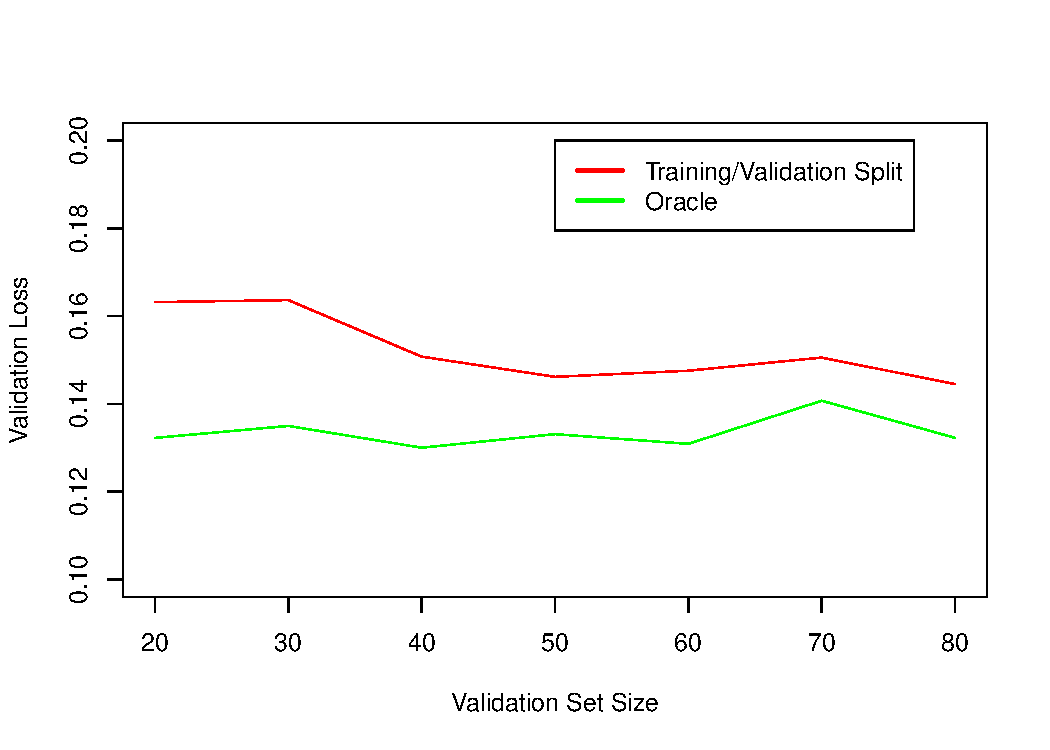
\includegraphics[height=80mm]{../R/figures/validation_size_loss.pdf}
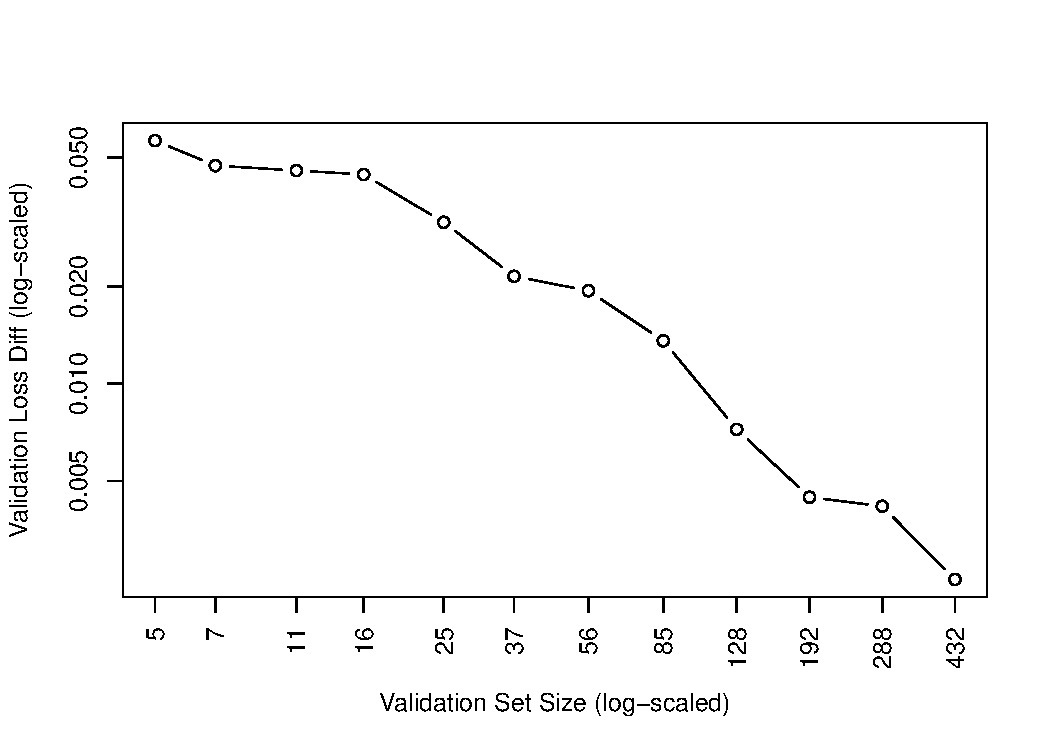
\includegraphics[height=80mm]{../R/figures/validation_size_loss_diff.pdf}
%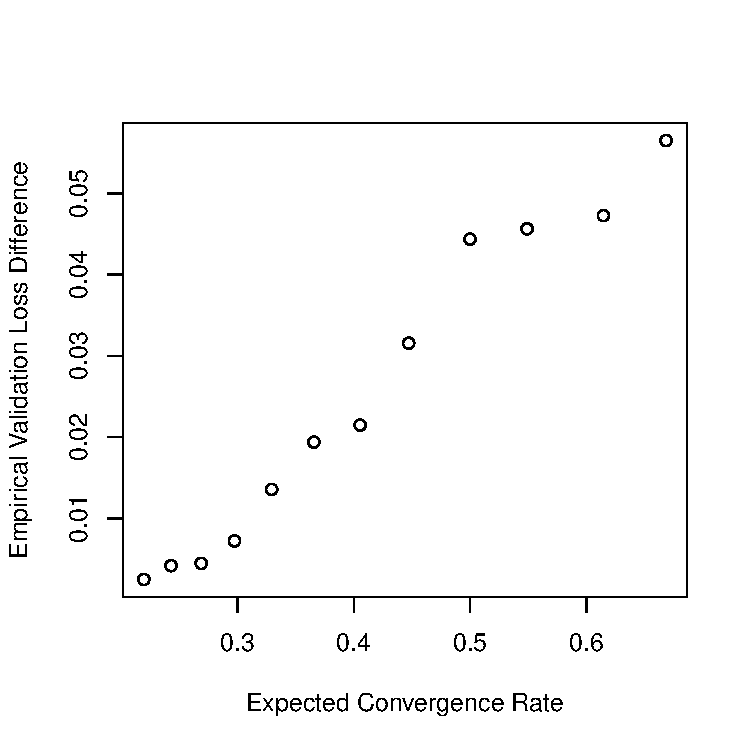
\includegraphics[height=80mm]{../R/figures/qqplot.pdf}
\end{figure}

\section{Discussion}\label{sec:discussion}

In this paper, we have shown that the difference in prediction error of the model chosen by cross-validation and the oracle model decreases at a near-parametric rate if the fitted models are smoothly parameterized in terms of the penalty parameters. For many penalized regression problems, we find that this is indeed the case. Our results show that adding penalty parameters does not drastically increase the model complexity. This supports recent efforts to combine regularization methods and ``un-pool" regularization parameters. Furthermore, since our result holds for a search over a dense set of penalty parameters, our prediction error bounds apply to cross-validation over a continuum of values, as done in hyper-parameter optimization methods.

The main caveat is that our theorems bound the prediction error of the global minimizer of the validation set. However this is hard to achieve practically since the validation loss is not convex in the penalty parameters. More investigation needs to be done to bound the prediction error of fitted models that are local minima.

A different approach we could have taken in this paper is to bound the distance between the estimated and oracle penalty parameters
\begin{equation}
\label{penalty_diff}
\left \| \hat{\boldsymbol \lambda} - \tilde{\boldsymbol \lambda} \right \|_2
\end{equation}
instead of the fitted values. Bounding \ref{penalty_diff} is not obvious from the definitions of $\hat{\boldsymbol{\lambda}}$ and would probably require more regularity assumptions on the model class. However, it could provide a more intuitive understanding of the behavior of cross-validation-like procedures.

\section{The Proof} \label{sec:proofs}

In this paper, we will measure the the complexity of $\mathcal{G}(T)$ by its metric entropy. Let us recall its definition here:

\begin{definition}
Let the covering number $N(u, \mathcal{G}, \| \cdot \|)$ be the smallest set of $u$-covers of $\mathcal{G}$ with respect to the norm $\| \cdot \|$. The metric entropy of $\mathcal{G}$ is defined as the log of the covering number:
\begin{equation}
H (u, \mathcal{G}, \| \cdot \| ) = \log N(u, \mathcal{G}, \| \cdot \|)
\end{equation}
\end{definition}

\begin{theorem}
\label{train_val_thrm_complicated}
Let $\epsilon$ be independent sub-Gaussian random variables.
Suppose that $\sup_{g \in \mathcal{G}} \| g \|_\infty \le G < \infty$.
Suppose for any training dataset $T \subseteq D$ with $\| \epsilon \|_T \le 2 \sigma$, we have
\begin{equation}
\int_0^R H^{1/2} \left ( u, \mathcal{G(\cdot | T)} \| \cdot \|_V \right ) du \le \psi(n, J, \sigma)
\end{equation}

Then for all $\delta  > 0$ such that
\begin{equation}
\sqrt{n_{V}}\delta^{2}
\ge
c \left[
\psi_{T}\left(2\left\Vert \hat{g}_{\tilde{\lambda}}-g^{*}\right\Vert _{V} + 2\delta\right)
\vee
\left(2\left\Vert \hat{g}_{\tilde{\lambda}}-g^{*}\right\Vert _{V}+2\delta\right)
\right]
\end{equation}

Then with high probability, we have
\begin{equation}
\left \|\hat{g}_{\hat{\lambda} }(\cdot | T) - g^* \right \|_V
\le
\min_{\lambda \in \Lambda}\| \hat{g}_{\lambda}(\cdot | T) - g^*\|_V
+ \delta
\end{equation}
\end{theorem}

\begin{proof}
Chaining and peeling.
\end{proof}

%In the penalized regression setting, each function $\hat{g}(\cdot |\boldsymbol \lambda)$ in $\mathcal{G}(T)$ directly maps to a set of penalty parameters, so one would expect that the covering number of $\mathcal{G}(T)$ and $\Lambda$ to be related. In Section \ref{sec:entropy}, we show that $\hat{g}(\cdot | \boldsymbol \lambda)$ is smoothly parameterized by $\boldsymbol \lambda$ in many penalized regression problems. Using this result, we apply Theorem \ref{train_val_thrm_complicated} to the specific case of penalized regression to get Theorem \ref{train_val_thrm}.
%
%Note that the complexity term in the upper bound contains a $\log n_V$ term. This is the result of allowing the range of $\Lambda$ to increase at a polynomial rate in the validation set size $n_V$. (Perhaps we should be more explicit and just have $\lambda_{\min} $ and $\lambda_{\max}$)

\paragraph{Proof of Theorem \ref{train_val_thrm}}

\begin{proof}
%By Lemma param\_covering\_cube, we have
%\[
%H(u,\mathcal{G}(T),\|\cdot\|_{V})\le\log\frac{1}{C_{J}}+J\log\left(\frac{2n^{t_{max}-\kappa}+2Cu}{Cu}\right)
%\]
%
%
%Let $R_{1}=R\wedge\sqrt{n^{t_{max}-\kappa}/C}$.
%
%Then after immense algebraic massaging, we get
%\begin{equation}
%\int_{0}^{R}H{}^{1/2}(u,\mathcal{G}(T),\|\cdot\|_{V})du
%\le
%R\left(\left[\log\frac{1}{C_{J}}+J(2+\log4)+J\log\left(\frac{4n^{t_{max}-\kappa}}{C}\right)\right]^{1/2}+\sqrt{2J\log\frac{1}{R}\vee0}\right)
%\end{equation}
%
%We note since $\delta > \frac{1}{n_{V}}$ (modulo a constant), it suffices to choose $\delta$ such that
%\[
%\sqrt{n_{V}}\delta^{2}\ge c\left(\left\Vert \hat{g}_{\tilde{\lambda}}-g^{*}\right\Vert _{V}+\delta\right)\left(\left[\log\frac{1}{C_{J}}+J(1+\log4)+J\log\left(\frac{4n^{t_{max}-\kappa}}{C}\right)\right]^{1/2}+\sqrt{J\log n_{V}}\right)
%\]
%
%Let
%\[
%K=c\left(\left[\log\frac{1}{C_{J}}+J(1+\log4)+J\log\left(\frac{4n^{t_{max}-\kappa}}{C}\right)\right]^{1/2}+\sqrt{J\log n_{V}}\right)
%\]
%and
%\[
%\omega=\left\Vert \hat{g}_{\tilde{\lambda}}-g^{*}\right\Vert _{V}
%\]
%
%The quadratic formula gives us that
%\[
%\delta\ge\frac{K+\sqrt{K^{2}+4K\omega\sqrt{n_{V}}}}{2\sqrt{n_{V}}}
%\]
\end{proof}



\paragraph{Proof of Theorem \ref{kfold_thrm}}

\begin{lemma}
\label{oracle_maintained}
The oracle rate isn't changed when we add the ridge penalty
\end{lemma}

\paragraph{Proof of Lemma \ref{lemma:smooth}}
\paragraph{Proof of Lemma \ref{lemma:nonsmooth}}

\paragraph{Proof of Lemma \ref{lemma:parametric}}

\begin{lemma}
\label{lemma:sobolev_prop}
Sobolev penalty has nice properties
\end{lemma}

\paragraph{Proof of Lemma \ref{lemma:sobolev}}

\bigskip

\bibliographystyle{agsm}
\bibliography{multi-penalties-theory}

\end{document}
